\addcontentsline{toc}{section}{Materials and Methods}
\section*{Materials and Methods}

%%%%%%%%%%%%%%%%%%%%%%%%%%%%%%%%%%%%%%%%%%%%%%%%%%%%%%%%%%%%%%%%%%%%%%%
\phantomsection
\addcontentsline{toc}{subsection}{Study Site}
\subsection*{Study Site}

\begin{itemize}
    \item 50-ha long term forest monitoring plot
    \item central Panama
    \item (lat, lon)
    \item moist lowland tropical predominantly evergreen forest, only 10\% of canopy drops leaves during the dry season %\citep{condt_2000} 
    \item mean annual precipitation of $2662 \pm 479$ (SD) mm yr$^{(-1)}$ and a 4-month dry season ($<$ 100 mm per month)  
    \item average annual rainfall of about 2640 mm (Detto et al.,
2018) and a well-marked dry season (total rainfall between late-December and mid-April is about 175 mm on average). 
    \item Why is BCI a good choice for this study?
\end{itemize}
%%%%%%%%%%%%%%%%%%%%%%%%%%%%%%%%%%%%%%%%%%%%%%%%%%%%%%%%%%%%%%%%%%%%%%%
\phantomsection
\addcontentsline{toc}{subsubsection}{Initial Vegetation Conditions}
\subsection*{Initial Conditions}

\paragraph{BCI 2012 survey data}
After establishment in 1981 in 1981, species and dbh of all living trees $<$ 1 cm have been inventoried every 5 years since 1985 \citep{condit_1995}. 

\paragraph{Soil} 
Soil data?

%%%%%%%%%%%%%%%%%%%%%%%%%%%%%%%%%%%%%%%%%%%%%%%%%%%%%%%%%%%%%%%%%%%%%%%
\addcontentsline{toc}{subsubsection}{Atmospheric Conditions}
\subsection*{Atmospheric Conditions}

\paragraph{Choosing Simulation Period}

% \begin{wrapfigure}{!r}{0.45\textwidth}
%     \centering
%     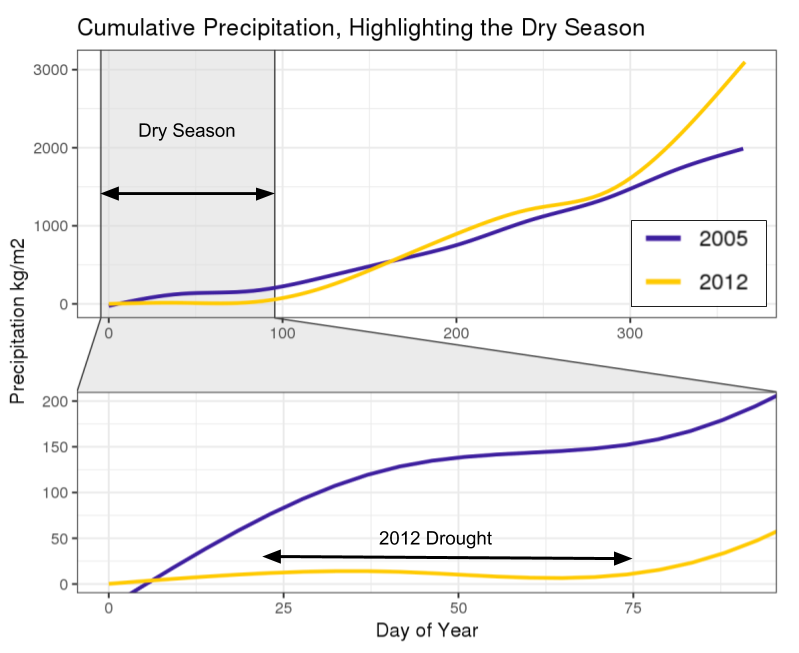
\includegraphics[width=.45\textwidth]{Hydro_Paper_LaTeX/Hydro_Paper_Figures/precip.png}
%     \caption[Precipitation]{Precipitation: To be more informative, this plot should also have the average of all the available years to get a better idea of how "extreme" these two scenarios actually are.}
%     \todoa{caption}
%     \label{fig:precip}
% \end{wrapfigure}

\begin{figure}[!h]
    \centering
    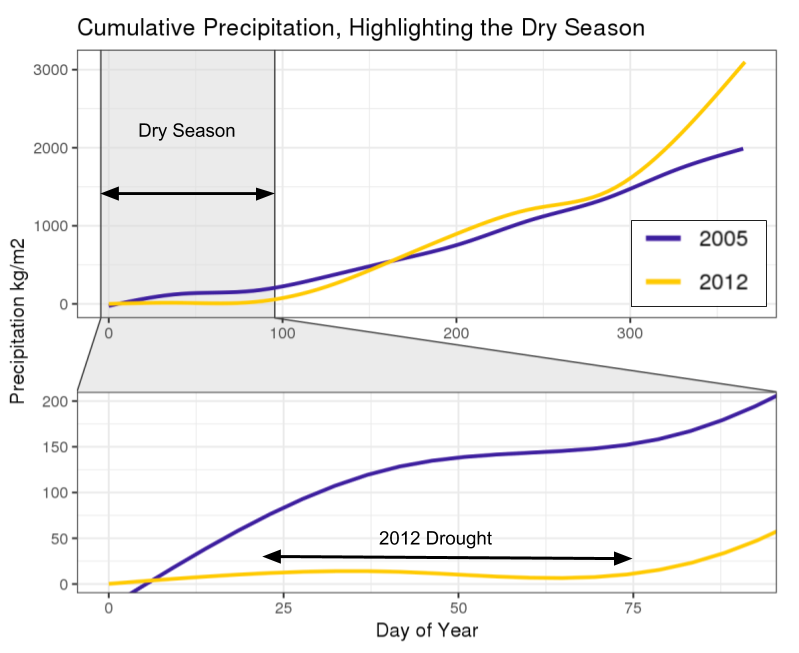
\includegraphics[width=.65\textwidth]{Hydro_Paper_LaTeX/Hydro_Paper_Figures/precip.png}
    \caption[Precipitation]{Cumulative precipitation at Barro Colorado Island, Panama for the years 2012 (yellow) and 2005 (purple). The pictured years have the most divergent climactic conditions over the dry season, with 2012 having an dry and prolonged dry season and 2005 having a short and wet dry season. 
    \todoq{To be more informative, this plot should also have the average of all the available years to get a better idea of how "extreme" these two scenarios actually are.}}
    % \todoa{caption}
    \label{fig:precip}
\end{figure}



 Meteorological data of the simulated years were available at hourly resolution for air temperature, wind speed, specific humidity, precipitation rate, short- and longwave radiation, and were hence used as ecosystem upper boundary condition. 
 
 Two years were chosen to represent the two extremes in the avaialable data: the shortest and wetest dry season and the longest and dryest dry season, which  
 
 % I should ask Felicien about CO2 ... To exclude CO2 fertilization effects and keep the same meteorological drivers as in our previous study (di Porcia e Brugnera et al., 2019), the atmospheric concentration of CO2 was fixed at a constant value of 370 ppm, which corresponds to initial concentrations measured by the flux towers.

%%%%%%%%%%%%%%%%%%%%%%%%%%%%%%%%%%%%%%%%%%%%%%%%%%%%%%%%%%%%%%%%%%%%%%%
\addcontentsline{toc}{subsection}{Ecosystem Demography Model Version 2.2}
\subsection*{Ecosystem Demography Model (Version 2.2)}

\begin{figure}[h]
    \centering
    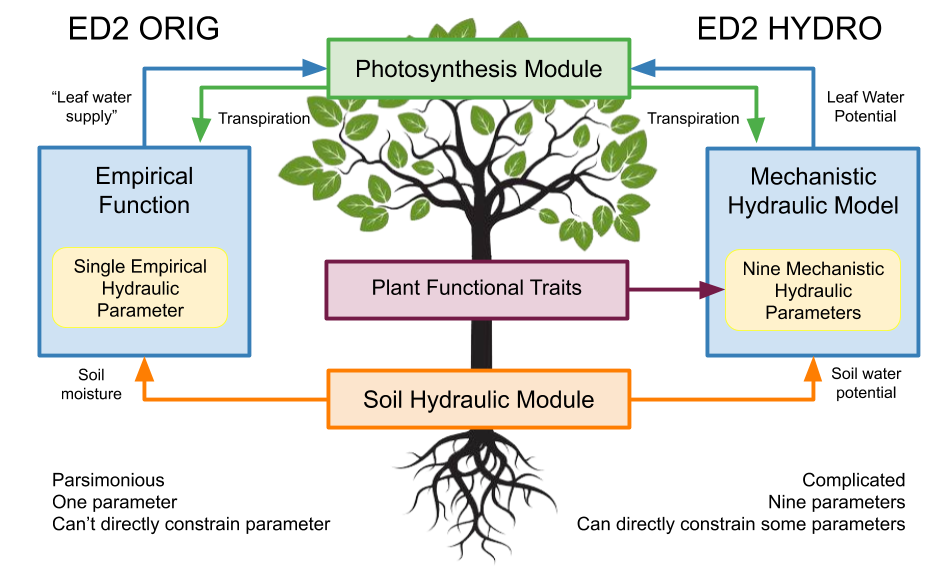
\includegraphics[width=.75\textwidth]{Hydro_Paper_LaTeX/Hydro_Paper_Figures/ED_versions.png}
    \caption[ED2 versions]{ED2 vs ED2-hydro}
    \label{fig:ED_versions}
\end{figure}

Because ED2 is a DGVM, it uses the dynmaics of PFTs. Thus we need to talk about how we define PFTs. 

\begin{itemize}
    \item In this case, plant functional types (PFTs) are defined as a collection of species. 
    \item These species are cross-listed with a database of plant traits. 
    \item This data can then be used to constrain probability distributions that define our apriori knowledge of the parameter values for the plant traits in question. 
    \item To initialize parameter values for a model run in ED, a Bayesian meta-analysis is performed in which posterior distributions are calculated for each model parameter value included in the analysis, and then values are randomly selected from the distribution. Note that the current meta-analys system does not allow for joint distribution sampling. 
    \item The scope of this study is to focus on the propagation of parameter uncertainly over small timescale processes, competition between PFTs was not included. Thus, the PFT used is a general tropical PFT, consisting of the combination of early, mid and late species.
\end{itemize}

\begin{itemize}
    \item ED2-hydro Tropical PFT: http://psql-pecan.bu.edu/bety/pfts/1000000131
    \item ED2 TropicalPFT: http://psql-pecan.bu.edu/bety/pfts/1000000132
    \item The PFTs are based on clones of a FATES prior, and then species were added in during the meta-analysis. Should I discuss this process?
\end{itemize}

%%%%%%%%%%%%%%%%%%%%%%%%%%%%%%%%%%%%%%%%%%%%%%%%%%%%%%%%%%%%%%%%%%%%%%%
%%%%%%%%%%%%%%%%%%%%%%%%%%%%%%%%%%%%%%%%%%%%%%%%%%%%%%%%%%%%%%%%%%%%%%%
\newpage
\addcontentsline{toc}{subsection}{Attributing Uncertainty to Ecological Processes}
\subsection*{Attributing Uncertainty to Ecological Processes}

\phantomsection
\addcontentsline{toc}{subsubsection}{The Predictive Ecosystem Analyser}
\subsubsection*{PEcAn}

- What are the most current PEcAn papers for describing the uncertaintly analysis workflow? Add Lebauer to the bib!


\addcontentsline{toc}{subsubsection}{Calculating Parameter Uncertainty}
\subsubsection*{Calculating Parameter Uncertainty}

Look how mike explains his uncertainty analysis in his papers. Also the author that starts with Z 2015, Also Felicien's paper, also Koven 2020. 

\paragraph{Meta Analysis}

\begin{itemize}
    \item Non-hydraulic trait data: BETY database 
    \item Hydraulic trait data: Felicien's paper  
    \item Leaf biomass allometry trait data: BAAD database
    \item root data from authors I need to add
    \item check for additional data I need to add to data list
    \item BETYdb citation
\end{itemize}

% \begin{itemize}
%     \item Parameter
%     \item Prior
%     \item a
%     \item b
%     \item Prior meadian
%     \item ED2 defaulthttps://www.overleaf.com/project/5ecf1a2873cb7e00019c95ab
%     \item Posterior median
%     \item N (sample size)
%     \item $\text{CV}_{\text{p,posterior}}/\text{CV}_{\text{p,prior}}$
% \end{itemize}

%Please add the following packages if necessary:
%\usepackage{booktabs, multirow} % for borders \& merged ranges
%\usepackage{soul}% for underlines
%\usepackage[table]{xcolor} % for cell colors
%\usepackage{changepage,threeparttable} % for wide tables

%If the table is too wide, replace \begin{table}[!htp]...\end{table} with
%\begin{adjustwidth}{-2.5 cm}{-2.5 cm}\centering\begin{threeparttable}[!htb]...\end{threeparttable}\end{adjustwidth}
\begin{table}[!htp]\centering
\caption{Table of Parameters (Do we want this table to also include distributions?)}\label{tab:params}
\scriptsize
\begin{tabular}{lrrcc|rrrr}\toprule
Trait &Proccess(es) &Units &ED2 &ED2-hydro &Prior distribution &Param a &Param b \\\midrule
Leaf Turgor Loss Point &Hydraulics & &- &+ & & & \\
Leaf Water Cap &Hydraulics & &- &+ & & & \\
Root Beta &Hydraulics & &- &+ & & & \\
Specific Root Area &Hydraulics & &- &+ & & & \\
stoma_psi_c &Hydraulics & &- &+ & & & \\
Kexp &Hydraulics & &- &+ & & & \\
Kmax &Hydraulics & &- &+ & & & \\
Wood Turgor Loss Point &Hydraulics & &- &+ & & & \\
p50 &Hydraulics & &- &+ & & & \\
Wood Water Cap &Hydraulics & &- &+ & & & \\
Water Cond. &Hydraulics & &+ &- & & & \\
Abvgnd \% Struc. Biomass &Allocation \& Allometry & &+ &+ & & & \\
Leaf Biomass Allom. Int. &Allocation \& Allometry & &+ &+ & & & \\
Root Depth Allom. Int. &Allocation \& Allometry & &+ &+ & & & \\
Leaf Biomass Allom. Slope &Allocation \& Allometry & &+ &+ & & & \\
Root Depth Allom. Slope &Allocation \& Allometry & &+ &+ & & & \\
Fine Root Allocation &Allocation \& Allometry & &+ &+ & & & \\
Specific Leaf Area &Allocation \& Allometry & &+ &+ & & & \\
Wood Density &Allocation \& Allometry & &+ &+ & & & \\
Quantum Efficiency &Photosynthesis \& Stomatal Cond. & &+ &+ & & & \\
Stomatal Slope &Photosynthesis \& Stomatal Cond. & &+ &+ & & & \\
Vcmax &Photosynthesis \& Stomatal Cond. & &+ &+ & & & \\
Leaf NIR reflectance &Radiation & &+ &+ & & & \\
Leaf VIS reflectance &Radiation & &+ &+ & & & \\
Leaf NIR transmittance &Radiation & &+ &+ & & & \\
Leaf VIS transmittance &Radiation & &+ &+ & & & \\
Leaf orientation &Radiation & &+ &+ & & & \\
Growth Respiration &Respiration \& Turnover & &+ &+ & & & \\
Leaf Respiration Rate &Respiration \& Turnover & &+ &+ & & & \\
Leaf Turnover Rate &Respiration \& Turnover & &+ &+ & & & \\
Root Turnover Rate &Respiration \& Turnover & &+ &+ & & & \\
Veg. Resp. Q10 &Respiration \& Turnover & &+ &+ & & & \\
\bottomrule
\end{tabular}
\end{table}

\begin{figure}[!h]
    \centering
    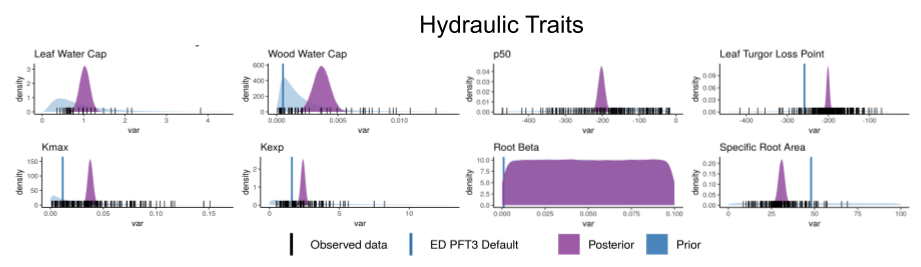
\includegraphics[width=.95\textwidth]{Hydro_Paper_LaTeX/Hydro_Paper_Figures/hydraulic_traits.png}
    \caption[Hydraulic Traits]{Parameter distributions for ED2-hydro PFT in the BETY database. Prior distributions (blue) were constrained by data from BETYdb (not pictured, though in the final version of the plot I do want to have data points) using Bayesian meta-analysis to produce posterior distributions (purple). In two cases there was no data to constrain the prior and thus the posterior remains uninormative. The dashed dark blue line shows the default value for ED2-hydro's mid-successional tropical PFT.
    \todoq{Because my PFT is a combination of early, mid and late, would it be useful or clutter to have all three PFT default lines on the plot? Are the default lines useful at all?}
    }
    \label{fig:hydraulic_traits}
\end{figure}


\addcontentsline{toc}{subsubsection}{Calculating Parameter Sensitivity and Contribution to Model Uncertainty}
\subsubsection*{Calculating Parameter Sensitivity and Contribution to Model Uncertainty}

\paragraph{Sensitivity Analysis and Variance Decomposition}

\addcontentsline{toc}{subsubsection}{Benchmarking}
\subsubsection*{Benchmarking}

\todoq{
This part of the analysis hasn't really been developed yet. Koven 2020 cites Detto 2018 as having observational eddy-covariance data such as GPP, LH, SH as well as observations of LAI.

Some form of model validation would be important to show that ED2-hydro is in fact making reasonable predictions while simultaneously reducing predictive variability. However, especially given \citep{powell_2018} showing the strength in ED2-hydro's predictive performance at this very site, I don't feel a particular need to spend a lot of time on benchmarking in this paper (also this takes time!). I'd like to hear other opinions on this. }